\documentclass[11pt, aspectratio=169, table]{beamer}
  % papersize={16cm,9cm},

\mode<presentation>{}

%%%%%%%%%%%%%%%%%%%%%%%%%%%%%%
% load packages
% add packages if needed

%\usepackage[T1]{fontenc}
\usepackage[utf8]{inputenc}
\usepackage{xcolor}
\usepackage[english]{babel}
\usepackage{amsmath,amsfonts,amssymb,amsthm}
\usepackage{color}
\usepackage[tracking=smallcaps, letterspace=-55]{microtype} % package for font spacing
\usepackage[outline]{contour}
%\usepackage[perpage]{footmisc}
\usepackage{transparent} % for setting opacity of pictures
\usepackage{pifont} % for checkmark (\ding{51}) and cross (\ding{55})
\usepackage{booktabs,array} % for tables
\usepackage{graphicx} % for figures
\usepackage{tikz}
\usepackage{pgfpages}
\usepackage{ulem}
\usepackage{dirtytalk}

%\graphicspath{} % to set the path of figures

\usetikzlibrary{shapes.multipart,positioning,matrix,external,shadows}

\renewcommand{\thefootnote}{\fnsymbol{footnote}}
\renewcommand{\thempfootnote}{\fnsymbol{mpfootnote}}

%\setbeameroption{show notes on second screen=bottom}

%%%%%%%%%%%%%%%%%%%%%%%%%%%%%%
% Fill in the following information: AUTHOR, TITLE, DATE

\author[Saska Dönges]{Saska Dönges}
\title[PfP intro]{Programming for Performance}
\subtitle{Intro lecture}
\date{March 16. 2024, BSCS2011}%{\today}
\institute{Dept.\ of Computer science, University of Helsinki
}

%%%%%%%%%%%%%%%%%%%%%%%%%%%%%%
% set beamer colors

\definecolor{hyblue}{RGB}{0,155,255}
\setbeamercolor{alerted text}{fg=hyblue}
\setbeamercolor{structure}{fg=hyblue}

\setbeamertemplate{itemize item}{\color{hyblue}}

%%%%%%%%%%%%%%%%%%%%%%%%%%%%%%
% set font (helvetica plays the role of Arial)
\usepackage{helvet}
\renewcommand{\familydefault}{\sfdefault}

%%%%%%%%%%%%%%%%%%%%%%%%%%%%%%
% set frametitle

\setbeamercolor{frametitle}{fg=black}%{fg=hyblue}
\setbeamerfont{frametitle}{series=\bfseries, shape=\scshape, size=\huge}
\setbeamertemplate{frametitle}[default][left,leftskip=3.5cm] % left shift of frame title
\addtobeamertemplate{frametitle}{\vspace{0.5cm}}{\vspace{1cm}} % spacing above and below frame title

%%%%%%%%%%%%%%%%%%%%%%%%%%%%%%
% set footline and headline
\beamertemplatenavigationsymbolsempty
\setbeamertemplate{headline}{ }
\setbeamertemplate{footline}{%
	 \usebeamercolor[fg]{page number in head/foot}%
	 \usebeamerfont{page number in head/foot}%
	\hspace{0.5cm}	
	
\includegraphics[width=2.5cm]{HY__LC05_txt__L_3L_B3____BW_cropped}
	\hfill
	\insertshorttitle\ /\ \insertshortauthor	\hfill
	\insertdate	\hspace{0.5cm}
	\insertframenumber\,/\,\inserttotalframenumber \hspace{0.5cm} \vskip2pt%
}

%%%%%%%%%%%%%%%%%%%%%%%%%%%%%%
% Other style settings
\useinnertheme{circles}

%%%%%%%%%%%%%%%%%%%%%%%%%%%%%%
% For video
\usepackage{media9}%
\newcommand{\includemovie}[3]{%
\includemedia[%
width=#1,height=#2,%
activate=onclick,%
deactivate=pageclose,%
addresource=#3,%
flashvars={%
src=#3 % same path as in addresource!
%&autoPlay=true % default: false; if =true, automatically starts playback after activation (see option ‘activation)’
&loop=true % if loop=true, media is played in a loop
&controlBarAutoHideTimeout=0 %  time span before auto-hide
}%
]{}{StrobeMediaPlayback.swf}%
}

%%%%%%%%%%%%%%%%%%%%%%%%%%%%%%
%%%%%%%%%%%%%%%%%%%%%%%%%%%%%%

\begin{document}

%% Title slide with HY picture
%{
%\usebackgroundtemplate{
%\setlength{\unitlength}{1cm}
%\begin{picture}(16,9)
%\transparent{0.33}
%\put(0.3,0.8){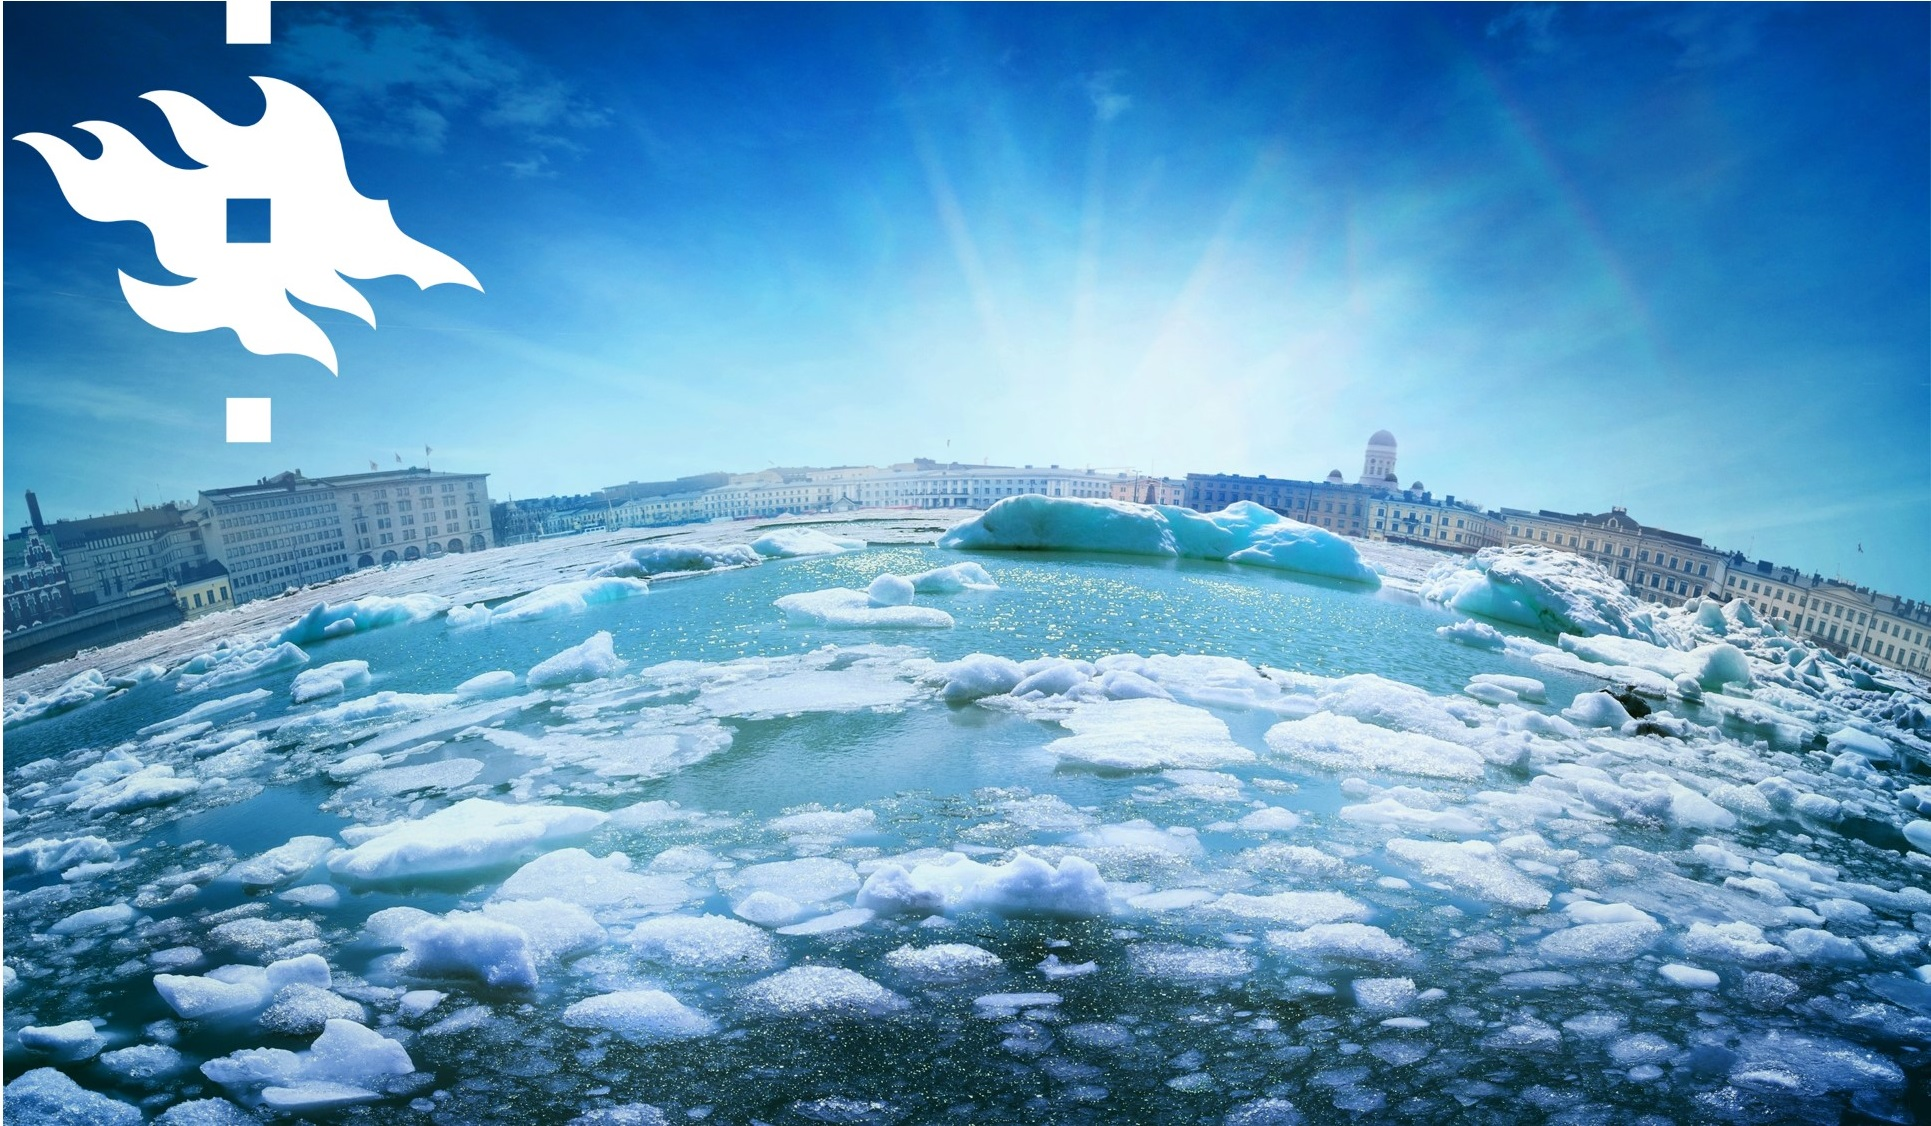
\includegraphics[width=15cm,height=7.8cm]{hy_brand_image_1_wide_background_hires_logo} }
%\end{picture}
%}
%\setbeamertemplate{headline}{ }%
%\begin{frame}{}
%\vspace{2.5cm}
%\begin{center}
%\huge
%{\bf \inserttitle } \\
%{\large \insertauthor}
%\end{center}
%\end{frame}
%}



% Title page without picture
{
\usebackgroundtemplate{
\setlength{\unitlength}{1cm}
\begin{picture}(16,9)
	\put(-0.1,5){ 
\includegraphics[width=4cm]{HY__LA01_Flame_____B3____BW} }
\end{picture}
\setlength{\unitlength}{1pt}
}
\setbeamertemplate{headline}{ }%
\begin{frame}[noframenumbering]{}
\vspace{2.5cm}
\begin{center}
\huge
\textcolor{hyblue}{ \bf
\inserttitle
} \\
{\large
\insertauthor}
\end{center}
\end{frame}
}
%

%%%%%%%%%%%%%%%%%%%%%%%%%%%%%%
%% Main text

%% set HY Logo on the upper-left corner:
\usebackgroundtemplate{
\setlength{\unitlength}{1cm}
\begin{picture}(16,2.5)
\put(0.1,0){

\includegraphics[width=2.5cm]{HY__LA01_Flame_____B3____BW}\hfill
}
\end{picture}
\setlength{\unitlength}{1pt}
}
%%

%%%%%%%%%%%%%%%%%%%%%%%%%%%%%%
%% Modify text below

\begin{frame}{Agenda}
\setlength\parskip{\fill}
\tableofcontents
\alert{Interrupt} to comment or ask questions!
\end{frame}

\section{Goals}
\begin{frame}{After todays lecture you should...}
\begin{itemize}
\itemsep=\fill
\item know how the course is sructured,
\item know what is required of you to pass the course
\item and have a basic understanding of some of the higher level concepts explored on the course.
\end{itemize}
\end{frame}

\section{Introductions and probing questions.}
\begin{frame}{Who am I? Who are you?}
\begin{itemize}
	\itemsep=\fill
	\item Where from (BSc, CS, Math, Physics)?
	\item What for?
	\item Course history?
	\item Relevant supporting knowledge?
\end{itemize}
\end{frame}

\begin{frame}{This course...}
\setlength\parskip{\fill}
...is a replacement for the \alert{OLD} course ``Programming in C''. A self-guided, 
automatically assessed C Programming course.

...now has a fancyer name and a skew towad performance. (Beyond the addition of ``++''.)

...aims to give you all programming practice in C++, and an awareness of some issues affecting
performance and ways to improve performance.
\end{frame}

\begin{frame}{Do this, do that}
\setlength\parskip{\fill}
There is lots of C++ on the web -- by all
means learn from it, but \alert{NO CHEATING!!!}

Engage in \alert{difficult study} in order to develop
your ability to think so that your \alert{life becomes
easier}.
\end{frame}

\section{Course practicalities.}
\begin{frame}{Grading and assignments}
\setlength\parskip{\fill}
Final course grade is based on:
\begin{itemize}
	\item A series programming assignments,
	\item B series programming assignments,
	\item written assignments, and
	\item lecture / exercise session / case study activity.
\end{itemize}

To pass you will also need to have done 50\% of A series programming tasks and written 
assignments, as well as either actively attend at least 3 course meetings or pass an oral 
examination.
\end{frame}

\begin{frame}{Grading}
There are over 160 points available on the course. At least 40 points for each of the different
activity types. Initital point limits are as follows:
\begin{description}
\item{{\bf 0-39 points:}} grade 0
\item{{\bf 40-59 points:}} grade 1
\item{{\bf 60-79 points:}} grade 2
\item{{\bf 80-99 points:}} grade 3
\item{{\bf 100-119 points:}} grade 4
\item{{\bf 120+ points:}} grade 5
\end{description}

This is the second course implementation with this set of activieties, the initial grading criteria 
are still not guaranteed to be very good. The given point limits may lower, but will not under any 
circumstances be higher than this.
\end{frame}

\begin{frame}{``A'' series programming tasks}
\setlength\parskip{\fill}
Intended to be doable for people not particularly familiar with C++ or systems programming.

Main challenges should be:
\begin{itemize}
	\item working with C++,
	\item implementing software based on techincal descriptions and
	\item becoming familiar with concepts presented on the course.
\end{itemize}

If your implementations perform as required asymptotically, time and space limits should not be much of a concern.

I will be making spot checks to CSES submissions. No cheating!
\end{frame}

\begin{frame}{``B'' series programming tasks} 
\setlength\parskip{\fill}
Meant to be challenging.

I will make performance requirements as difficult as I can without making problems unfair.

Some tasks may still be very hard. Don't get discouraged if you can'c complete some B series tasks.

I don't expect many (any?) people to solve all of the B series tasks.

You don't technically need to solve any to get grade 5 on the course.
\end{frame}

\begin{frame}{Written tasks}
\setlength\parskip{\fill}
Written tasks are meant to push students in the direction of performance oriented thinking.

All written tasks are submitted to moodle.

For students not present at the exercise session following the assignment deadline, the submission will be 
manually graded by the TA (or me). (Feedback is not guaranteed)

For students present at the exercise session, self-reported points will be given by default, and TA will be making 
spot checks to verify that the self reported points and moodle submissions agree.
\end{frame}


\begin{frame}{Meeting activity}
There will be 3 kinds of meetings during the course:
\begin{description}
	\item{{\bf Lectures.}} Flipped classroom with pre-assignments.
	\item{{\bf Case studies.}} Discussion on specific problems with pre-assignments.
	\item{{\bf Exercise sessions.}} Discussing / presenting solutions to written assignments.
\end{description}

For each meeting (except the intro lecture), 4 points will be available for meeting activity.

Unfortunately, there are too many people enrolled for me to be able to give activity points without book-keeping.

A list will be circulated at the start of each meeting, and I will make note of activity on the attendence sheet
\end{frame}

\begin{frame}{Questions and comments?}
\setlength\parskip{\fill}
Do you disagree with how this course is run?

Do you have questions about course practicalities?
\end{frame}

\begin{frame}{Moodle}
\setlength\parskip{\fill}
Now is the time to switch to the browser.

Hope I remembered to set it up before.
\end{frame}

\section{Short break / Pre-assignment panic.}
\begin{frame}{Pre-assignment and break}
\setlength\parskip{\fill}
Hopefully I remembered to show the pre-assignment on moodle.

If you didn't realize that there was a pre-assignment you will now have until the end of the break to try to get up to speed.
\end{frame}

\section{High level discussion about course contents / Intro to PfP.}
\begin{frame}{What is systems programming?}
\setlength\parskip{\fill}
\pause
According to Wikipedia

\say{[T]he activity of programming computer system software. The primary distinguishing characteristic of systems programming 
when compared to application programming is that application programming aims to produce software which provides services 
to the user directly, whereas systems programming aims to produce software and software platforms which provide services to other 
software, are performance constrained, or both.}
\end{frame}

\begin{frame}{How is systems programming relevant for this course?}
\setlength\parskip{\fill}
\pause
While not completely accurate, systems programming is the best description for what we do on the course (that I can think of).

\pause
Specifically, we don't really care about user interfaces (graphical or otherwise), as long as we can control execution enough to 
run tests.

If someone were to ever actually use the code produced on this course, it would be as a data structure library or to get inspiration from
the implementation. Not to run the software as is.
\end{frame}

\begin{frame}{So what do we actually do?}
\setlength\parskip{\fill}
Beyond learning C++.\pause

Single thread, performance oriented data structures and supporting algorithms.
\end{frame}

\begin{frame}{What don't we do}
\setlength\parskip{\fill}\pause
Competetive programming. ``Algoritmit ongelmanratkaisussa'' (Algorithmic problem solving), by Antti laaksonen.

Cluster computing. ``Tools for high performance computing'' at the physics department.

Parallel computation. ``Programming parallel computers'' by Antti Laaksonen, from Aalto.
\end{frame}

\begin{frame}{What else we don't do}
\setlength\parskip{\fill}\pause
Real time systems. Theory is covered on operating systems and computer architecture courses, and perhaps something practical 
on the Networks study track.

Process Cohabitation on a single core / thread / system. Theory is somewhat covered on other courses, but nothing practical (AFAIK).

Actual low level programming. Writing device drivers or programming in assembly. Perhaps something on the Networks study track?
\end{frame}

\begin{frame}{Why C++}
\setlength\parskip{\fill}\pause
The vast majority of systems / low level code has been and is still written in C, C++ or fortran (if you are physics inclined).

The vast majority of all research code is written in C++, Python, fortran, Matlab or JavaScript

Since C++ is a superset(\alert{ish}) of C, and C++ is more convenient, we use C++ over C.

Since we aren't physicists (at least I'm not), we skip fortran.
\end{frame}

\begin{frame}{Why not $\langle$language$\rangle$?}
\begin{columns}
\begin{column}{0.5\textwidth}
\begin{itemize}
	\item Python
	\item Matlab
	\item JavaScript
	\item ASM
\end{itemize}
\end{column}
\begin{column}{0.5\textwidth}
\begin{itemize}
	\item Rust
	\item Java
	\item C\#
	\item ...
\end{itemize}
\end{column}
\end{columns}
\end{frame}

\section{Exit questionnaire.}
\begin{frame}{Questionnaire for course development and research}
\begin{columns}
\begin{column}{0.4\textwidth}
\setlength\parskip{1em}
\url{https://elomake.helsinki.fi/lomakkeet/128673/lomake.html}

It would really help me if you take the time to respond.
\end{column}
\begin{column}{0.6\textwidth}
\begin{center}

\includegraphics[width=0.5\columnwidth]{elomakeqr}
\end{center}
\end{column}
\end{columns}
\end{frame}

%{
%\usebackgroundtemplate{
%\transparent{0.3} % requires \usepackage{transparent} & compile twice
%\setlength{\unitlength}{1cm}
%\begin{picture}(16,9)
%\put(0.2,1){
%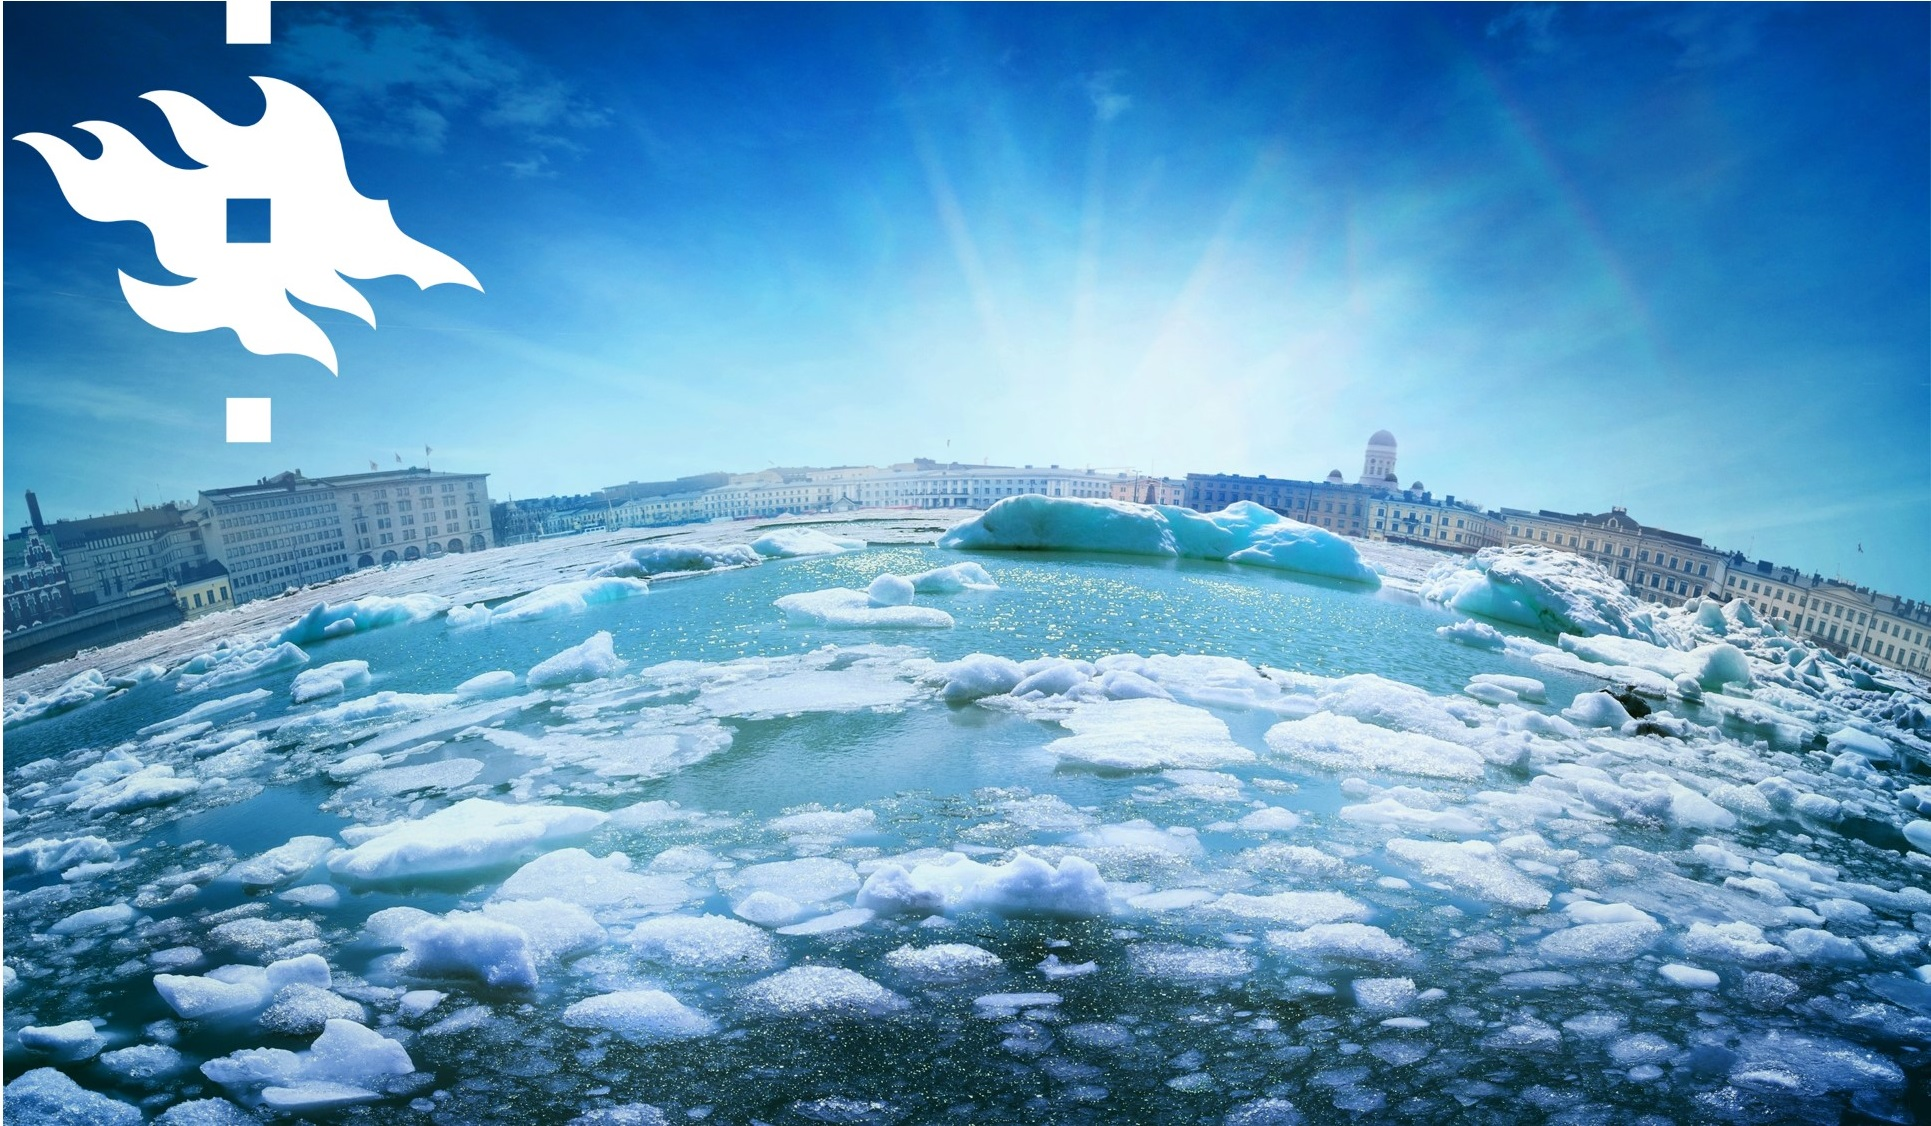
\includegraphics[width=15cm,height=7.5cm]{hy_brand_image_1_wide_background_hires_logo}
%}
%\end{picture}
%\setlength{\unitlength}{1pt}
%}
%
%\begin{frame}{\vspace{3cm}That's it}
%\begin{center}
%\vspace{-4cm}{\huge Questions?}
%\end{center}
%\end{frame}
%}

\end{document}





